%!TEX root = ../template.tex
%%%%%%%%%%%%%%%%%%%%%%%%%%%%%%%%%%%%%%%%%%%%%%%%%%%%%%%%%%%%%%%%%%%
%% chapter3.tex
%% NOVA thesis document file
%%
%% Chapter 3: Conceptual System Architecture (Technology-Agnostic)
%%%%%%%%%%%%%%%%%%%%%%%%%%%%%%%%%%%%%%%%%%%%%%%%%%%%%%%%%%%%%%%%%%%

\typeout{NT FILE chapter3.tex}%

\chapter{Conceptual System Architecture}
\label{cha:architecture}

This chapter presents the conceptual architecture, semantic data model, and interaction workflows of the proposed \gls{DT} framework. It defines the functional layers, interaction boundaries, and communication mechanisms connecting the physical shop floor to the virtual simulation. By decoupling simulation mechanics from operational asset data, the architecture allows industrial systems to evolve modularly while maintaining digital-physical alignment.

The remainder of this chapter is organized as follows:
\begin{itemize}
    \item \Cref{sec:design_requirements} defines the functional and non-functional requirements that guide the architectural design, along with their normative taxonomy and literature rationale.
    \item \Cref{sec:architecture_conceptual} introduces the conceptual architecture, outlining the core design principles, the upstream digitization stage (Layer~0), the operational activity workflows (Layers~1 to 3), and cross-layer interaction flows.
    \item \Cref{sec:asset_data_model} details the semantic metamodel, decomposing industrial assets into standardized submodels for 3D geometry, kinematics, \gls{IO} pin mappings, control logic, and network endpoints.
    \item \Cref{sec:architecture_summary} summarizes the conceptual architecture and provides the transition to the technological implementation.
\end{itemize}

\section{Design Requirements and Constraints}
\label{sec:design_requirements}

The design of a modular and automated \gls{DT} framework must address several key limitations identified in the State of the Art (\Cref{cha:stateoftheart}). Current industrial \glspl{DT} are often held back by tight coupling between 3D assets and proprietary simulation tools, slow manual synchronization pipelines, and a lack of vendor-neutral semantic interoperability \cite{Alexopoulos2025,Schaper2025}. At the same time, the transition toward \glspl{RMS} and \glspl{CPPS} requires plug-and-produce capabilities, allowing machines and stations to be added, swapped, or rearranged without costly downtime or manual re-engineering \cite{Rocha2024}.

Following the specification methodology of \textcite{Alemao2022}, requirements are organized into two main categories:
\begin{itemize}
    \item \textbf{Functional Requirements (FR):} Define the concrete actions, functions, and behaviors the system must perform, as well as its interactions with users and external services. They represent what the software architecture must execute.
    \item \textbf{Non-Functional Requirements (NFR):} Define the quality attributes, constraints, and operating boundaries of the system. Rather than describing specific features, they specify how well the system must perform in areas such as latency, scalability, fault isolation, and usability.
\end{itemize}

To clearly define the necessity of each requirement, this work adopts the modal taxonomy used by \textcite{Alemao2022}:
\begin{itemize}
    \item \textbf{‘‘Shall’’:} Mandatory and strictly required for system compliance.
    \item \textbf{‘‘Should’’:} Recommended feature or architectural intention that is desirable, but whose absence does not compromise basic compliance.
    \item \textbf{‘‘May’’:} Optional capability that provides additional flexibility without affecting core execution.
\end{itemize}

Based on these principles and the gaps identified in the literature, the functional and non-functional requirements are defined below:

\subsection{Functional Requirements}

\begin{enumerate}
    \item[\textbf{FR1}] \textbf{Plug-and-Play Asset Onboarding:} The framework shall support the registration and deployment of new industrial assets into the active ecosystem without requiring recompilation or manual changes to simulation software. Each asset shall be independently described, validated, and onboarded without disrupting running operations \cite{Rocha2024,AshtariTalkhestani2019}.

    \item[\textbf{FR2}] \textbf{Self-Describing Asset Packages:} All information needed to configure and execute a \gls{DT} shall be bundled into a single, standardized, and portable package per asset. This archive shall encapsulate 3D visual geometry, kinematic degrees of freedom, virtual sensor/actuator pin mappings, network endpoints, and behavioral control rules \cite{Lu2025,Gollner2022}.

    \item[\textbf{FR3}] \textbf{Dynamic Scene Assembly:} The simulation engine shall construct the virtual environment procedurally at startup by querying a central semantic registry, removing the need for pre-built or hard-coded scene files. The virtual environment shall adapt its spatial layout dynamically to reflect all registered assets \cite{Alexopoulos2025}.

    \item[\textbf{FR4}] \textbf{Physical-Virtual Synchronization and Drift Mitigation:} During runtime, the virtual model shall maintain continuous, bidirectional state synchronization with physical equipment. The synchronization mechanism shall detect discrepancies between periodic telemetry frames and automatically apply drift correction to preserve physical-digital consistency \cite{Kritzinger2018,Tao2019}.
\end{enumerate}

\subsection{Non-Functional Requirements}

\begin{enumerate}
    \item[\textbf{NFR1}] \textbf{Low-Latency Telemetry:} Sensor state changes and actuation events from physical hardware should reach the simulation engine with minimal latency to ensure responsive and timely state replication.

    \item[\textbf{NFR2}] \textbf{Scalability and Modularity:} The central registry and storage services should support concurrent asset registrations and multiple simulation clients without performance degradation or architectural changes.

    \item[\textbf{NFR3}] \textbf{Layer Independence and Fault Isolation:} Architectural layers shall remain functionally decoupled through well-defined \gls{API} contracts. A disruption, restart, or failure in the modeling or repository layer shall not stop active real-time simulation or shop-floor execution.

    \item[\textbf{NFR4}] \textbf{Configuration Usability and Accessibility:} Creating and packaging a \gls{DT} asset descriptor should not require low-level programming skills. The framework should provide an intuitive, guided interface suitable for automation and shop-floor engineers.
\end{enumerate}

These requirements define the criteria that guide the three-layer conceptual architecture presented next.


\section{Architectural Overview}
\label{sec:architecture_conceptual}

Current industrial \gls{DT} implementations face several practical bottlenecks that limit their flexibility and scalability on the shop floor:

\begin{enumerate}
    \item \textbf{Monolithic Coupling and Engineering Overhead:} Most commercial simulation platforms bundle 3D geometry, kinematic definitions, control scripts, and communication drivers into a single proprietary project file \cite{Striffler2023,Koch2024}. When a shop-floor station is modified, such as adjusting the stroke of a pneumatic cylinder, changing a clamp, or moving a proximity sensor, the virtual model cannot adapt on its own. An engineer must reopen the simulation tool, manually edit the mechanics and signal links, and redeploy the scene. This manual maintenance creates significant downtime and makes rapid reconfiguration difficult.

    \item \textbf{Fragmented Engineering Data:} Machine specifications are usually split across different tools and file types. Mechanics are stored in \gls{CAD} files, electrical connections in circuit diagrams or spreadsheets, and control logic in \gls{PLC} programs \cite{Luder2020,Ahvanouee2025}. For instance, adding a new conveyor module requires manually matching \gls{PLC} \gls{IO} addresses with simulation tags and positioning the 3D meshes by hand. Without a standardized, self-contained asset format, these disconnected sources lead to configuration mistakes and prolonged setup times \cite{Gollner2022,Schaper2025}.

    \item \textbf{Network Latency and Channel Congestion:} Several experimental architectures send both heavy visual assets and real-time operational data across the same communication channel or \gls{API} endpoint \cite{Gil2024,Pajpach2023}. Downloading large 3D models while simultaneously streaming high-frequency sensor updates creates network delays and jitter. In fast assembly lines, delayed sensor readings cause the simulation to lag behind the physical equipment, creating positional drift and breaking synchronization \cite{Kritzinger2018}.

    \item \textbf{Lack of Simulation-Ready Models for Existing Machinery:} Many factories rely on brownfield equipment that either lacks 3D \glspl{DM} entirely or only has detailed manufacturing \gls{CAD} drawings \cite{Lee2014,Striffler2023}. These manufacturing files often contain thousands of internal details, such as screw threads or wiring harnesses, while lacking kinematic joints and local pivot axes. Loading such models directly into a real-time physics engine degrades rendering performance and prevents moving components from functioning correctly.
\end{enumerate}

To address these challenges, the framework separates the asset lifecycle into three conceptual layers, supported by an initial preparation stage (Layer~0), as shown in \Cref{fig:architecture_conceptual}:
\begin{itemize}
    \item \textbf{Layer~1 (Asset Modeling):} Prepares and semantically annotates modular asset packages.
    \item \textbf{Layer~2 (Storage and Registry):} Stores asset files and manages a central directory of network endpoints.
    \item \textbf{Layer~3 (Runtime Execution and Synchronization):} Procedurally builds the virtual scene, runs the physics engine, and synchronizes state with the physical machines.
\end{itemize}

\begin{figure}[htbp]
    \centering
    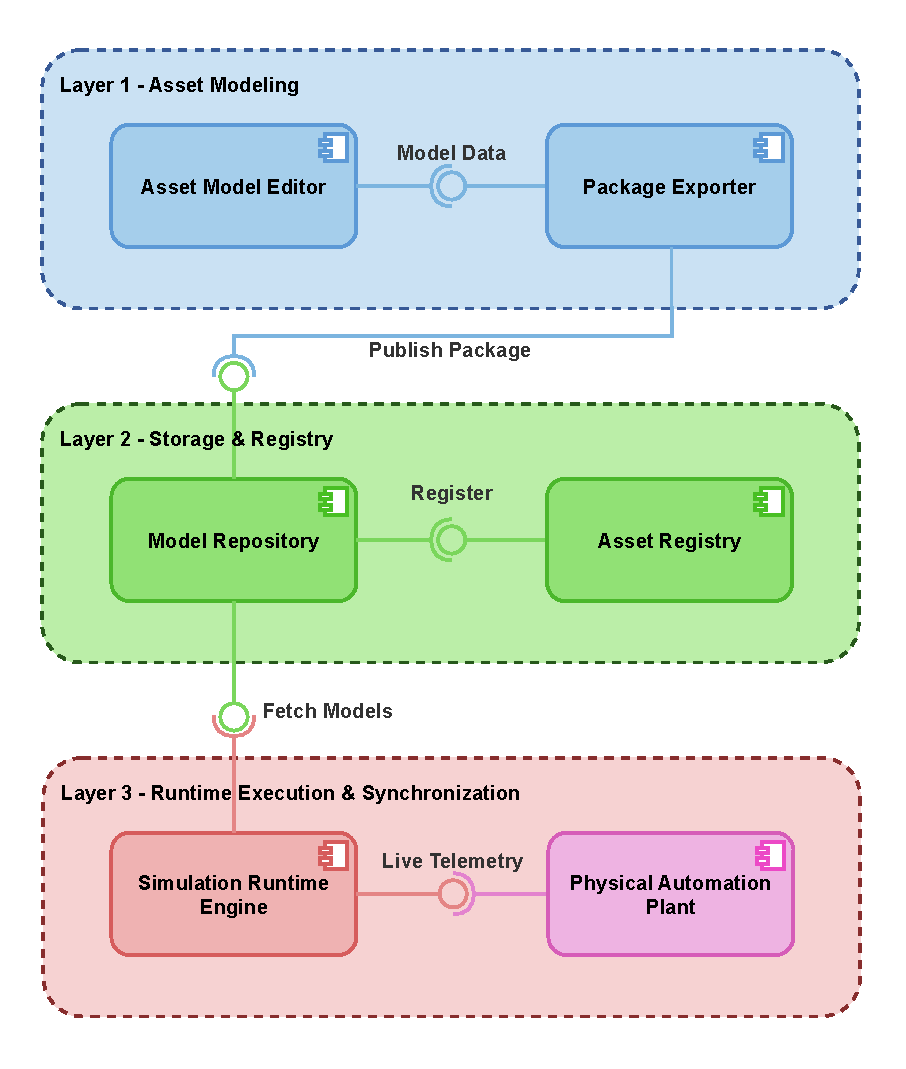
\includegraphics[width=\textwidth]{5-Figures/Arquitetura.drawio.pdf}
    \caption{Three-layer conceptual system architecture of the proposed \gls{DT} framework.}
    \label{fig:architecture_conceptual}
\end{figure}

The following subsections describe the role of each layer, the specific problems it solves, and how its components operate.

\subsection{Upstream Stage: Layer 0 - Physical Asset Digitization}
\label{sec:layer0_conceptual}

Before an industrial machine can be mirrored in software, the framework requires a clean geometric foundation. In an ideal greenfield project, machine builders supply lightweight, simulation-ready 3D models with pre-configured joints. In real factory environments, however, engineers typically face one of two negative extremes: either no digital 3D model exists at all, or the available \gls{CAD} files come directly from mechanical manufacturing. 

Manufacturing \gls{CAD} assemblies pose a major obstacle for real-time simulation. For example, a raw \gls{CAD} assembly of a pneumatic stamping station often contains internal screw threads, bearing balls, wiring, and dense solid geometry amounting to hundreds of thousands of polygons. Attempting to drop this raw file into a real-time graphics or physics engine causes severe frame drops. More critically, \gls{CAD} exports typically flatten all parts into a static hierarchy, stripping away the pivot points, motion axes, and stroke limits needed to simulate motion. Without properly configured local coordinate frames, a physics engine cannot determine whether a stamping rod is supposed to extend linearly or rotate around an arbitrary origin.

Layer~0 fills this gap by acting as the geometric preparation stage (\Cref{fig:layer0_conceptual}). Its objective is to produce a low-overhead, rigged 3D asset that accurately matches the physical dimensions of the equipment while discarding unnecessary internal complexity. 

The workflow relies on two main components:
\begin{enumerate}
    \item \textbf{3D Mesh Modeler:} Processes the raw mechanical \gls{CAD} model to produce a simulation-ready asset. Unnecessary internal details are removed, exterior surfaces are decimated to an efficient polygon budget, and basic collision boundaries are defined. Movable elements, such as pneumatic pushers, diversion gates, or rotating tables, are separated into independent sub-meshes, with their local coordinate frames and pivot points aligned directly with their functional axes of motion. Volumetric trigger zones (such as invisible box or cylindrical trigger colliders) are positioned at physical sensor locations, allowing the simulation engine to detect product passage or presence when parts enter these sensing volumes.
    \item \textbf{Model Exporter:} Exports the structured visual hierarchy, kinematics rigging, trigger zones, and materials into an open, vendor-neutral 3D binary format. This produces a lightweight, self-contained 3D geometry file ready for semantic authoring in Layer~1.
\end{enumerate}

\begin{figure}[htbp]
    \centering
    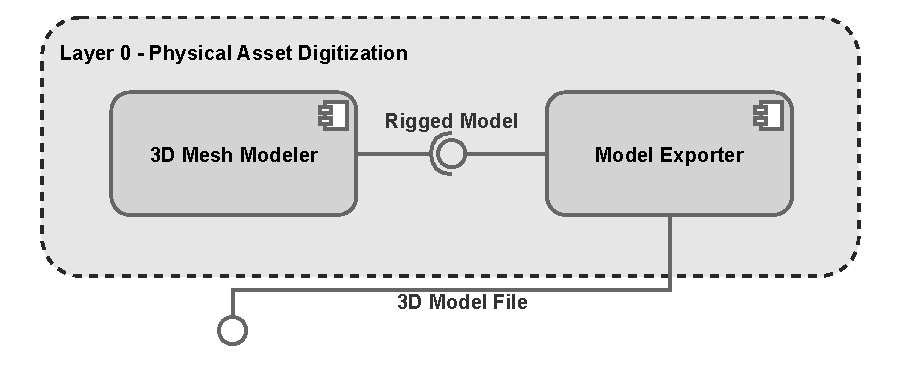
\includegraphics[width=0.7\textwidth]{drawio/layer0.pdf}
    \caption{\gls{UML} Component Diagram of Layer 0 (Physical Asset Digitization).}
    \label{fig:layer0_conceptual}
\end{figure}

Once the geometric boundaries, pivot points, and sensor trigger volumes are established in Layer~0, the resulting 3D asset provides the spatial foundation needed for operational configuration. However, this geometry contains no automation data. It must now enter Layer~1, where it is enriched with kinematics, electrical signals, and control logic.

\subsection{Layer 1 - Asset Modeling}
\label{sec:layer1_conceptual}

Layer~1 provides the authoring tools needed to transform static geometry into an operational \gls{DT} asset. A 3D model on its own is only a visual representation without any understanding of sensors, actuators, or control behavior. In conventional workflows, configuring these dynamics requires importing the model into a proprietary simulation suite and writing custom scripts inside that specific software.

This approach creates significant lock-in. When a factory changes its simulation software or attempts to connect multiple tools at once, all previous modeling and scripting work is lost. In addition, if a limit switch on the physical machine is rewired to another \gls{PLC} input terminal, an engineer has to search for the corresponding script in the simulation project and update it by hand. Operational data ends up scattered between electrical drawings, control logic, and simulation files.

Layer~1 resolves this fragmentation by keeping semantic modeling independent of any runtime engine. Its purpose is to combine visual geometry, kinematic limits, electrical pin mappings, and control rules into a standardized and portable asset package. 

The procedural workflow is illustrated in the \gls{UML} Activity Diagram in \Cref{fig:activity_layer1}, where the \textit{Asset Model Editor} and the \textit{Package Exporter} coordinate the process:
\begin{enumerate}
    \item \textbf{\gls{CAD} Import and Metadata Configuration:} The engineer imports the clean 3D file produced in Layer~0 into the \textit{Asset Model Editor} and assigns administrative metadata, including a unique global identifier, asset classification, and descriptive tags.
    \item \textbf{Kinematic Parsing and Joint Limits:} The \textit{Package Exporter} inspects the 3D transform hierarchy, identifies movable nodes, and allows the engineer to define their kinematic properties, including motion types, motion axes, and mechanical travel limits.
    \item \textbf{Virtual Pin Binding and Control Logic:} In the editor, the user defines the electrical and logical interface by creating virtual pins corresponding to physical controller \gls{IO} points. Sensor pins are anchored to detection zones to publish state changes upon product detection, while actuator pins drive the kinematic mechanisms when control commands are received. Local interlocking logic and communication topic bindings are assigned directly to these pins.
    \item \textbf{Validation and Package Compilation:} Before saving, the \textit{Package Exporter} validates the complete configuration against formal metamodel schemas, verifying that all declared pins and kinematic constraints are resolved. Once verified, it compiles the 3D geometry and descriptor files into a single, immutable asset package and publishes it to Layer~2.
\end{enumerate}

\begin{figure}[htbp]
    \centering
    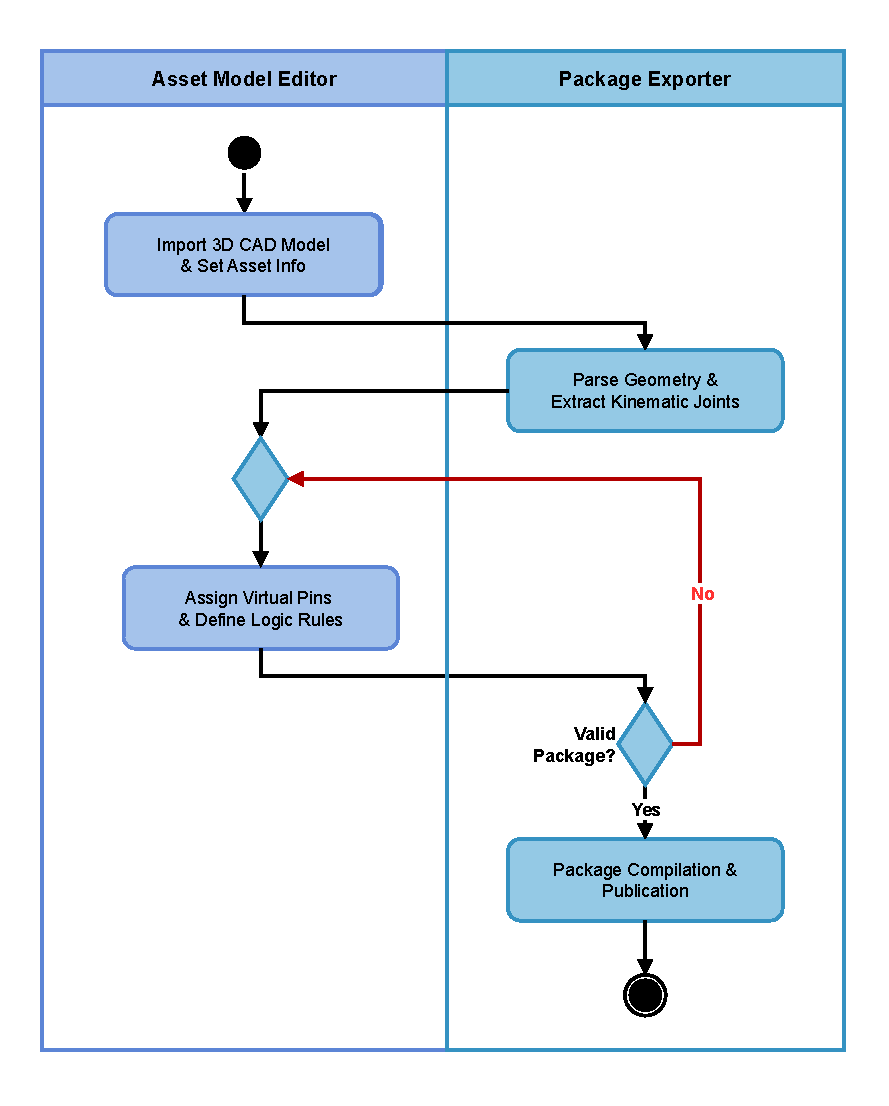
\includegraphics[width=0.85\textwidth]{drawio/assetmodeleditor.pdf}
    \caption{\gls{UML} Activity Diagram of Layer 1 (Asset Modeling).}
    \label{fig:activity_layer1}
\end{figure}

Compiling an asset package in Layer~1 completes the authoring pipeline for an individual machine. To make this self-contained package discoverable and accessible across the factory network, it is transferred to Layer~2, which hosts the repository and service directory.

\subsection{Layer 2 - Storage and Registry}
\label{sec:layer2_conceptual}

In a flexible or reconfigurable factory, machines and transport units are frequently rearranged, upgraded, or swapped out. In conventional simulation architectures, loading a modified layout requires an operator to manually copy new 3D model files onto every simulation computer, update local file paths, and re-enter static \gls{IP} addresses to connect to each machine's controller. 

This static approach breaks down quickly in agile production. For example, if an \gls{AGV} enters a production cell, or a faulty drilling station is replaced by a backup unit with different network settings, any simulation system relying on hard-coded addresses or local files stops working until someone manually reconfigures the environment. Mixing large file downloads with operational network queries often causes slow discovery responses and unnecessary network load.

Layer~2 acts as the central service directory and artifact distribution point for the entire \gls{DT} ecosystem. Its objective is to provide on-demand discovery and retrieval, allowing any authorized client on the factory network to locate active equipment, download corresponding models, and obtain the correct network topics automatically.

To keep discovery fast and scalable, Layer~2 separates heavy static files from dynamic directory metadata (illustrated in the \gls{UML} Activity Diagram in \Cref{fig:activity_layer2}) using two distinct services:
\begin{enumerate}
    \item \textbf{Model Repository:} Acts as a dedicated file store. It receives published asset packages from Layer~1, extracts the heavy 3D geometry meshes and descriptor schemas, and hosts them through standard \gls{HTTP} endpoints.
    \item \textbf{Asset Registry:} Functions as a lightweight service catalog. It records high-level metadata: the unique asset identifier, device classification, operational status, and active communication endpoints.
    \item \textbf{Dynamic Discovery and Provisioning:} When a simulation client starts up it queries the lightweight \textit{Asset Registry} via a \gls{REST} \gls{API} to find out which assets are available. The registry responds with the metadata and download URLs. Using these links, the client fetches the 3D geometry and submodels from the \textit{Model Repository}, loading them into memory without needing pre-installed local files.
\end{enumerate}

\begin{figure}[htbp]
    \centering
    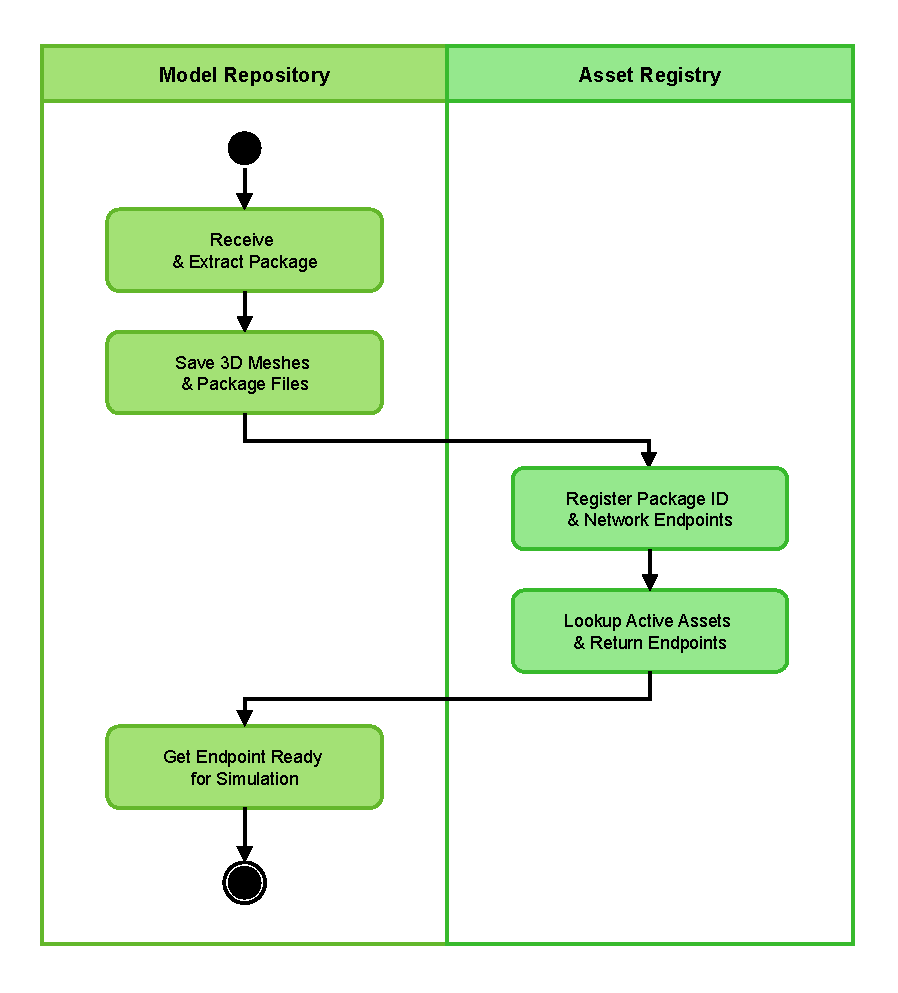
\includegraphics[width=0.85\textwidth]{5-Figures/Activity Storage and Registry.pdf}
    \caption{\gls{UML} Activity Diagram of Layer 2 (Storage and Registry).}
    \label{fig:activity_layer2}
\end{figure}

With the asset packages cataloged and network endpoints registered in Layer~2, the \gls{DT} models are ready to be consumed. Layer~3 interacts directly with Layer~2 to discover these assets and instantiate the runtime simulation.

\subsection{Layer 3 - Runtime Execution and Physical Synchronization}
\label{sec:layer3_conceptual}

The ultimate value of a \gls{DT} lies in running a faithful, real-time virtual counterpart that mirrors physical production without human intervention. In standard industrial setups, assembling a virtual cell requires opening a simulation editor, dragging and dropping machine models into place, manually positioning them, and setting up real-time drivers. 

Even after a virtual cell is configured, maintaining accurate physical-digital synchronization presents a major technical hurdle. Physics engines compute movements through discrete time steps using numerical approximations. If a virtual belt conveyor runs solely on simulated friction, slight timing variances and rounding errors accumulate over continuous operation. A workpiece on the virtual conveyor will slowly drift away from its true physical position, causing virtual sensors to trigger at incorrect times and resulting in false alarms or desynchronized simulation states. Conversely, attempting to stream high-detail geometric meshes across the same communication channel that carries cyclic sensor telemetry creates queueing bottlenecks, delaying critical sensor packets.

Layer~3 solves these problems by combining automated procedural scene generation with real-time state synchronization and drift correction. Its objective is to build the virtual environment dynamically at startup and maintain tight digital-physical alignment throughout production.

As shown in the \gls{UML} Activity Diagram (\Cref{fig:activity_layer3}), Layer~3 coordinates the runtime engine with the physical automation plant through parallel execution loops:
\begin{enumerate}
    \item \textbf{Procedural Scene Assembly:} When launched, the simulation runtime queries the Layer~2 registry, downloads the necessary asset packages, and reconstructs the virtual factory floor directly in memory. It automatically creates 3D visual nodes, binds physics colliders, assigns kinematic joint limits, and maps virtual pins based on the downloaded descriptors, requiring no manual scene editing.
    \item \textbf{Continuous Physics Simulation:} The simulation engine runs an internal physics loop at a steady frequency, calculating rigid-body collisions, gravity, and joint movements so that material handling and mechanical operations behave realistically.
    \item \textbf{Isolated Low-Latency Telemetry:} In parallel, the physical machines on the shop floor run their cyclic \gls{PLC} scan routines. When physical sensors or actuator states change, the controller sends compact telemetry packets over a dedicated, low-overhead messaging protocol straight to the simulation runtime, bypassing storage databases entirely to minimize delay.
    \item \textbf{State Updates and Drift Correction Snapping:} When the simulation receives an incoming telemetry packet, it updates the virtual sensor indicators and commands the virtual actuators. Because friction and contact physics accumulate small numerical errors over time, a moving workpiece will naturally drift away from its real position. To eliminate this divergence, each physical sensor detection acts as an absolute ground-truth reference point: the moment the hardware sensor trips, the simulation engine instantly snaps the virtual workpiece to the exact physical coordinates of that sensor before the next physics tick. This resets accumulated drift to zero and guarantees continuous physical-digital alignment even during extended production runs.
\end{enumerate}

\begin{figure}[htbp]
    \centering
    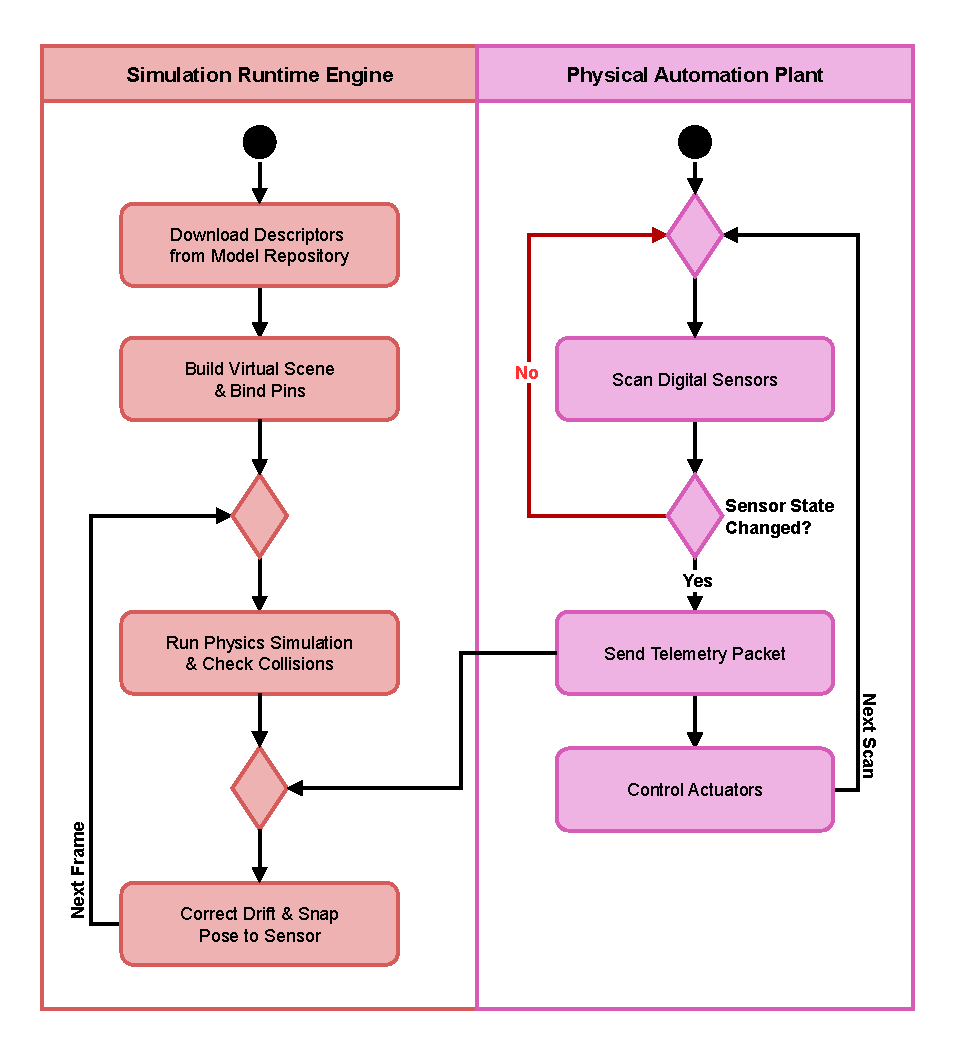
\includegraphics[width=0.85\textwidth]{5-Figures/activity_layer3.pdf}
    \caption{\gls{UML} Activity Diagram of Layer 3 (Runtime Execution and Physical Synchronization).}
    \label{fig:activity_layer3}
\end{figure}

\subsection{Cross-Layer Information and Interaction Flows}
\label{sec:architecture_flows}

While each architectural layer operates as an independent subsystem with its own lifecycle, the strength of the framework lies in how data moves across layer boundaries. In traditional monolithic simulation tools, engineering models, network configurations, and real-time signals are tightly bundled together, creating dependencies where changes in one domain require manual updates across the entire system.

To overcome this coupling, the proposed architecture coordinates three distinct communication flows, as shown in the conceptual overview in \Cref{fig:architecture_conceptual} (\cpageref{fig:architecture_conceptual}). These flows are separated by lifecycle phase, data volume, and timing constraints:

\begin{enumerate}
    \item \textbf{Asset Publication Flow (Design-Time: Layer~1 $\rightarrow$ Layer~2):} This flow takes place whenever an automation engineer authors or updates an asset. Because this exchange happens during engineering rather than production, latency is not critical. However, payload volume is relatively high, as it contains complete 3D meshes, collision data, and semantic submodel descriptors. The modeling tool packages these assets into an immutable archive, uploads the binary files to the \textit{Model Repository}, and registers the machine metadata and network endpoints in the \textit{Asset Registry}. Once published, the asset becomes immediately discoverable across the factory network.

    \item \textbf{Dynamic Ingestion Flow (Deployment-Time: Layer~2 $\rightarrow$ Layer~3):} This flow occurs on demand when a simulation instance starts up, or when a reconfigurable workstation enters the manufacturing cell. The runtime engine first queries the \textit{Asset Registry} using lightweight \gls{API} calls to discover which physical assets are currently present and operational. Guided by the registry responses, the engine requests the corresponding 3D geometry files and submodels from the \textit{Model Repository}. By constructing the virtual scene dynamically in memory, the system avoids pre-compiled scene files and ensures that any workstation newly added to Layer~2 is instantiated in simulation without restarting or re-engineering the application.

    \item \textbf{Low-Latency Telemetry Flow (Runtime: Physical Plant $\rightarrow$ Layer~3):} Unlike the previous two flows, which handle heavy descriptive data on an infrequent basis, the telemetry flow operates continuously during live production. When hardware sensors detect part movements or PLCs execute actuation cycles, state updates must reach the simulation engine with minimal delay. To achieve this, telemetry completely bypasses the storage and registry services of Layer~2. Instead, physical controllers publish compact, event-driven sensor packets directly to the simulation engine over a dedicated, low-overhead messaging channel. This separation protects real-time synchronization from network jitter, allowing the physics engine to apply drift correction and update virtual states deterministically.
\end{enumerate}

Segregating these three flows ensures that heavy model transfers never interfere with time-critical automation data. While this architectural division defines the functional boundaries and interaction patterns of the framework, executing these workflows requires a common, structured language to describe each machine. The following section defines the semantic data model that enables this cross-layer interoperability.

\section{Asset Data Model Specification}
\label{sec:asset_data_model}

To avoid relying on proprietary simulation tools, the framework defines a technology-neutral data model. The model standardizes how shop-floor machinery is described across all layers, separating visual 3D geometry, kinematics, \gls{IO} signals, local control logic, and network endpoints.

\Cref{fig:asset_metamodel_conceptual} shows the complete \gls{UML} Class Diagram of the conceptual asset metamodel. The root entity, \textit{AssetDescriptor}, brings together five submodel classes: \textit{VisualStructure}, \textit{BehaviorMapping}, \textit{VirtualPins}, \textit{NetworkEndpoint}, and \textit{ControlLogic}. All attributes use standard primitive types (\textit{String}, \textit{Float}, \textit{Integer}, \textit{Boolean}, and \textit{Vector3}, representing a 3D float coordinate or vector $(x, y, z)$).

\begin{figure}[htbp]
    \centering
    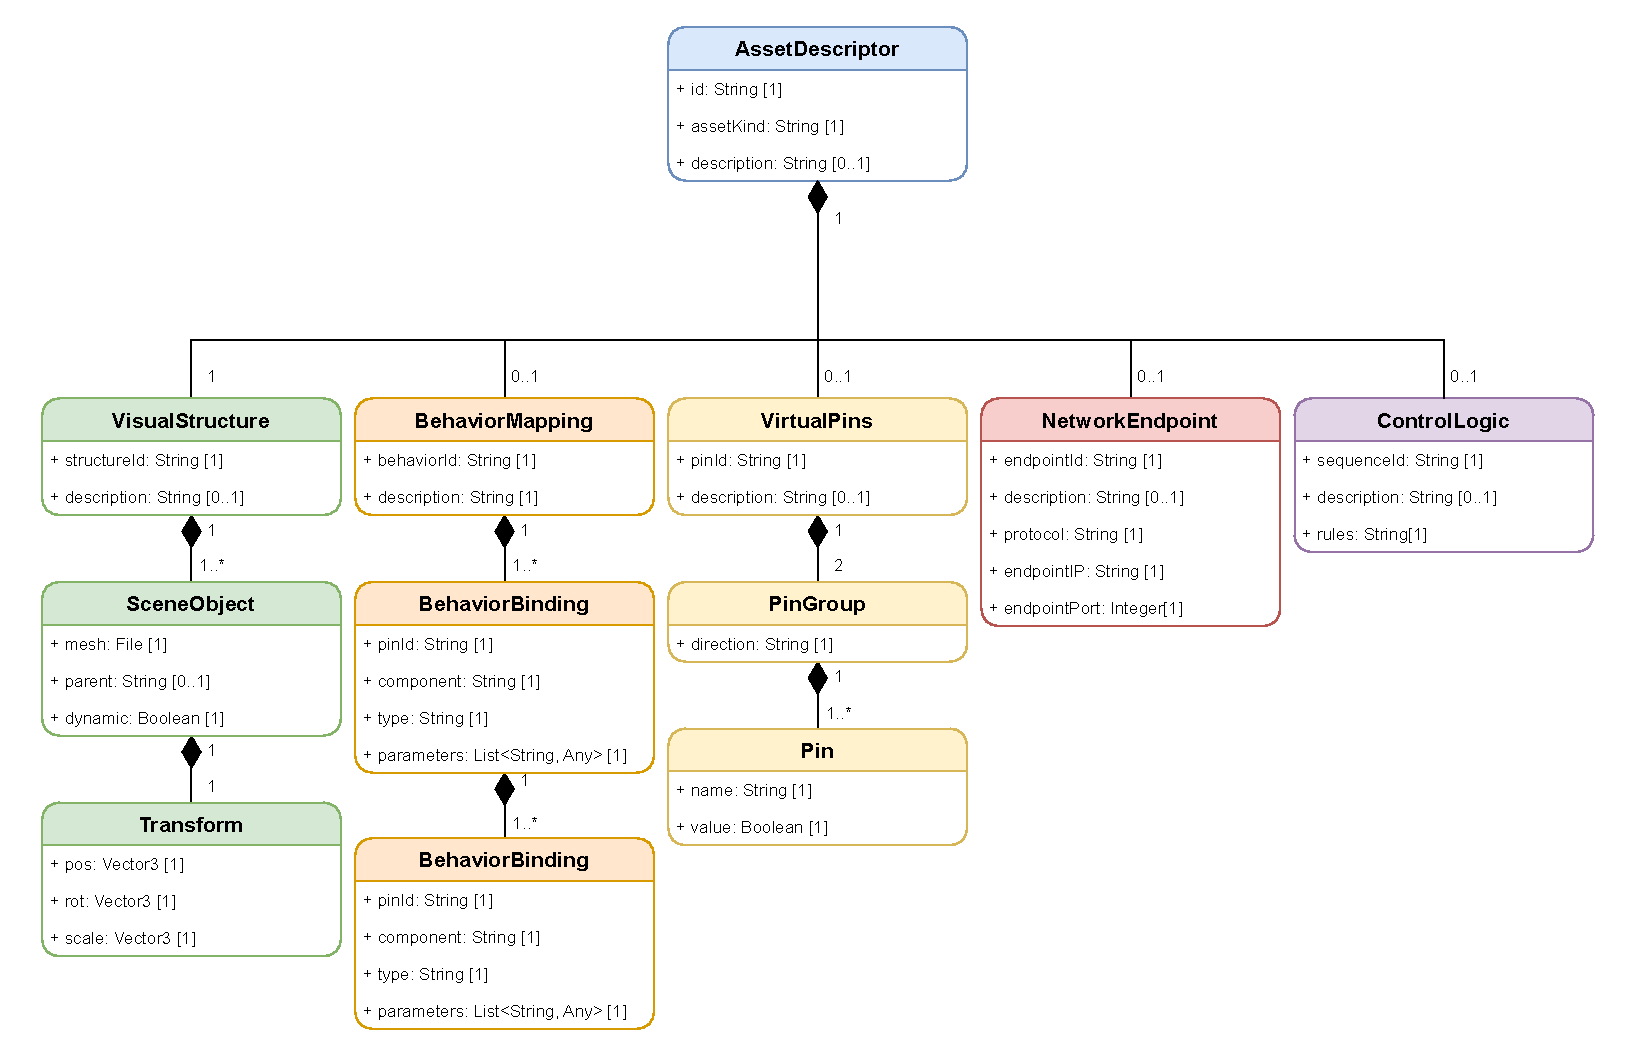
\includegraphics[width=\textwidth]{5-Figures/Modelo de Dados.drawio.pdf}
    \caption{\gls{UML} Class Diagram of the conceptual asset metamodel and constituent submodel classes.}
    \label{fig:asset_metamodel_conceptual}
\end{figure}

Each subsection below describes one class in detail, covering its purpose, multiplicity, and attributes.

\subsection{AssetDescriptor (Core Entity)}
\label{sec:model_asset_descriptor}

The \textit{AssetDescriptor} is the main container and identity root for any machine or workstation. It holds identity and classification data, acting as the entry point for registries and simulation parsers, as depicted in the \gls{UML} Class Diagram in \Cref{fig:metamodel_asset_descriptor}.

\begin{figure}[htbp]
    \centering
    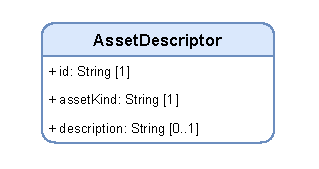
\includegraphics[width=0.4\textwidth]{5-Figures/AssetDescriptor.pdf}
    \caption{\gls{UML} Class Diagram of the core \textit{AssetDescriptor} entity.}
    \label{fig:metamodel_asset_descriptor}
\end{figure}

The attributes of \textit{AssetDescriptor} are:
\begin{itemize}
    \item \textbf{\textit{id}} (\textit{String}, $[1]$): A unique identifier used for naming, \glspl{UI}, and registry lookups.
    \item \textbf{\textit{assetKind}} (\textit{String}, $[1]$): The functional type or category of the machine.
    \item \textbf{\textit{description}} (\textit{String}, $[0..1]$): An optional text description of the machine.
\end{itemize}

\subsection{VisualStructure Class}
\label{sec:model_visual_structure}

The \textit{VisualStructure} class defines the 3D visual and spatial layout of an asset, independent of any particular graphics format. An \textit{AssetDescriptor} contains a single \textit{VisualStructure} submodel ($1$). Within this submodel, the asset defines a collection of one or more \textit{SceneObject} nodes ($1..*$), where each node carries exactly one \textit{Transform} ($1$). The structural organization of this hierarchy is illustrated in the \gls{UML} Class Diagram in \Cref{fig:metamodel_visual_structure}.

\begin{figure}[htbp]
    \centering
    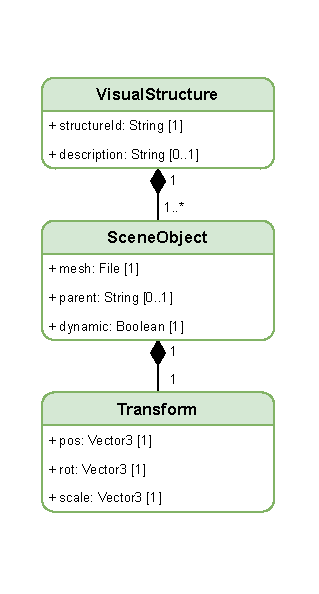
\includegraphics[width=0.4\textwidth]{5-Figures/VisualStructure.pdf}
    \caption{\gls{UML} Class Diagram of the \textit{VisualStructure} hierarchy (\textit{VisualStructure}, \textit{SceneObject}, and \textit{Transform}).}
    \label{fig:metamodel_visual_structure}
\end{figure}

The attributes in the \textit{VisualStructure} hierarchy are:

\textbf{\textit{VisualStructure}:}
\begin{itemize}
    \item \textbf{\textit{structureId}} (\textit{String}, $[1]$): The identifier of this visual group within the asset.
    \item \textbf{\textit{description}} (\textit{String}, $[0..1]$): An optional text description of the assembly.
\end{itemize}

\textbf{\textit{SceneObject}:}
\begin{itemize}
    \item \textbf{\textit{mesh}} (\textit{File}, $[1]$): The 3D surface mesh file for this node.
    \item \textbf{\textit{parent}} (\textit{String}, $[0..1]$): The identifier of the parent node, defining transform inheritance for multi-part assemblies.
    \item \textbf{\textit{dynamic}} (\textit{Boolean}, $[1]$): A flag indicating whether this component moves during operation.
\end{itemize}

\textbf{\textit{Transform}:}
\begin{itemize}
    \item \textbf{\textit{pos}} (\textit{Vector3}, $[1]$): The 3D position offset $(x, y, z)$ in meters relative to the parent frame.
    \item \textbf{\textit{rot}} (\textit{Vector3}, $[1]$): Euler angles $(\alpha, \beta, \gamma)$ in degrees (pitch, yaw, roll).
    \item \textbf{\textit{scale}} (\textit{Vector3}, $[1]$): Scale factors $(s_x, s_y, s_z)$, set to $(1.0, 1.0, 1.0)$ by default.
\end{itemize}

\subsection{BehaviorMapping Class}
\label{sec:model_behavior_mapping}

While 3D meshes define visual geometry, they do not inherently convey how a physical component operates or responds to automation signals. The \textit{BehaviorMapping} class bridges this gap by defining the operational behavior and kinematic properties of sensors and actuators ($0..1$). It encapsulates the domain configuration and physics parameters required by the simulation engine, grouping one or more \textit{BehaviorBinding} entries ($1..*$). 

The \textit{BehaviorMapping} class does not store the raw boolean signal values. Instead, it specifies how each component behaves during operation:
\begin{itemize}
    \item \textbf{For an Actuator:} It specifies the kinematic motion profile, vector of action, operating speed, stroke limits, and mechanical interaction with workpieces.
    \item \textbf{For a Sensor:} It defines the spatial detection boundary, target filtering criteria, electrical signal inversion logic, and synchronization snapping parameters.
\end{itemize}

Before inspecting the structure, the \gls{UML} Class Diagram in \Cref{fig:metamodel_behavior_binding} illustrates the class hierarchy for \textit{BehaviorMapping} and \textit{BehaviorBinding}.

\begin{figure}[htbp]
    \centering
    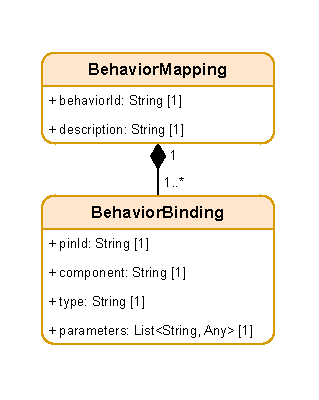
\includegraphics[width=0.4\textwidth]{5-Figures/BehaviorMapping.pdf}
    \caption{\gls{UML} Class Diagram of the \textit{BehaviorMapping} hierarchy (\textit{BehaviorMapping} and \textit{BehaviorBinding}).}
    \label{fig:metamodel_behavior_binding}
\end{figure}

The attributes across the \textit{BehaviorMapping} hierarchy (\Cref{fig:metamodel_behavior_binding}) are:

\textbf{\textit{BehaviorMapping}:}
\begin{itemize}
    \item \textbf{\textit{behaviorId}} (\textit{String}, $[1]$): Unique identifier for this behavioral profile within the asset descriptor.
    \item \textbf{\textit{description}} (\textit{String}, $[1]$): Functional description documenting the scope of the behavioral configuration.
\end{itemize}

\textbf{\textit{BehaviorBinding}:}
\begin{itemize}
    \item \textbf{\textit{pinId}} (\textit{String}, $[1]$): The identifier of the corresponding logical channel defined in \textit{VirtualPins} that drives or observes this component.
    \item \textbf{\textit{component}} (\textit{String}, $[1]$): The targeted \textit{SceneObject} node in \textit{VisualStructure} whose physical behavior is modulated by this binding.
    \item \textbf{\textit{type}} (\textit{String}, $[1]$): The functional mechanism category governing execution logic in the physics runtime, such as continuous linear or rotational conveyors (\textit{TranslateContinuous}, \textit{RotateContinuous}), mechanical linkages and joints (\textit{RotateHinge}, \textit{LinearCylinder}), or spatial detection volumes (\textit{TriggerZone}).
    \item \textbf{\textit{parameters}} (\textit{List$\langle$String, Any$\rangle$}, $[1]$): Dynamic dictionary of operational configuration settings. Rather than enforcing rigid sub-classing for every physical mechanism, this attribute is modeled as an extensible key-value collection. This preserves backward compatibility while accommodating both actuators and sensors:
    \begin{enumerate}
        \item \textbf{Actuator Parameters:}
        \begin{itemize}
            \item \textbf{\textit{AxisX, AxisY, AxisZ}} (\textit{Double}, $[1]$): Normalized direction vector defining the linear line of action or rotational axis, expressed in the local coordinate frame of the target node.
            \item \textbf{\textit{Speed}} (\textit{Double}, $[1]$): Velocity magnitude driving the continuous linear surface displacement or angular articulation rate.
            \item \textbf{\textit{RealPortID}} (\textit{String}, $[1]$): Physical terminal designation or register address on the field controller, linking the abstract virtual channel to physical hardware.
            \item \textbf{\textit{RealActuatorEnabled}} (\textit{Boolean}, $[1]$): Operational routing flag determining whether actuation commands dispatch to physical hardware or execute exclusively within the virtual simulation.
            \item \textbf{\textit{Visible}} (\textit{Boolean}, $[1]$): Flag specifying whether actuation directional gizmos or bounding outlines are rendered in the viewport.
        \end{itemize}

        \item \textbf{Sensor Parameters:}
        \begin{itemize}
            \item \textbf{\textit{TargetFilter}} (\textit{String}, $[1]$): Classification tag defining which moving colliders are eligible to trip the sensor volume, preventing false positives from static structures or irrelevant fixtures. For instance, an inductive or magnetic proximity sensor can be configured to detect only workpieces tagged as metallic or magnetic, ignoring non-magnetic plastic carriers.
            \item \textbf{\textit{ActiveLow}} (\textit{Boolean}, $[1]$): Electrical polarity flag specifying whether the logical state represents normally open or normally closed physical sensor contact behavior.
            \item \textbf{\textit{RealPortID}} (\textit{String}, $[1]$): Physical terminal designation or register address on the field controller from which telemetry originates.
            \item \textbf{\textit{RealSensorEnabled}} (\textit{Boolean}, $[1]$): Operational routing flag indicating whether runtime execution receives live field telemetry or runs under local virtual simulation.
            \item \textbf{\textit{Visible}} (\textit{Boolean}, $[1]$): Flag controlling whether the volumetric sensing boundary is visually rendered as a debug wireframe during execution.
            \item \textbf{\textit{SensingRange}} (\textit{Double}, $[0..1]$): Geometric radius or volumetric dimension defining the extent of the detection zone.
            \item \textbf{\textit{MoveTarget}} (\textit{String}, $[0..1]$): Identifier of the target scene component, movable fixture, or detected object whose spatial coordinates are subject to realignment upon sensor state change.
            \item \textbf{\textit{MoveOnState}} (\textit{Boolean}, $[0..1]$): Signal transition edge (rising versus falling transition) that triggers kinematic pose snapping.
            \item \textbf{\textit{MoveMode}} (\textit{String}, $[0..1]$): Correction scope applied to the target component upon triggering, selecting whether the runtime aligns spatial coordinates (\textit{Position Only}), angular orientation (\textit{Rotation Only}), or both degrees of freedom simultaneously (\textit{Position and Rotation}).
            \item \textbf{\textit{MovePosX, MovePosY, MovePosZ}} (\textit{Double}, $[0..1]$): Target local 3D coordinates $(x, y, z)$ to which the component is instantly repositioned, establishing an exact positional reference at the triggering event.
            \item \textbf{\textit{MoveRotX, MoveRotY, MoveRotZ}} (\textit{Double}, $[0..1]$): Target Euler orientation angles $(\alpha, \beta, \gamma)$ applied to adjust component alignment, eliminating accumulated angular deviation.
        \end{itemize}
    \end{enumerate}
\end{itemize}

\subsection{VirtualPins Class}
\label{sec:model_virtual_pins}

In contrast to \textit{BehaviorMapping} (which defines behavioral characteristics and kinematic kinematics), the \textit{VirtualPins} class models the pure electrical \gls{IO} interface of the asset ($0..1$). It acts as the digital image of physical controller terminals or fieldbus communication tags, abstracting raw hardware addresses into standardized discrete channels.

Each \textit{VirtualPins} instance contains two dedicated \textit{PinGroup} collections categorized by data direction (\textit{INPUT} and \textit{OUTPUT}). Each group contains the individual \textit{Pin} instances representing discrete boolean states ($1..*$).

To illustrate the relationship between terminals, signal direction, and individual channels, the \gls{UML} Class Diagram in \Cref{fig:metamodel_signal_interface} details the \textit{VirtualPins} hierarchy.

\begin{figure}[htbp]
    \centering
    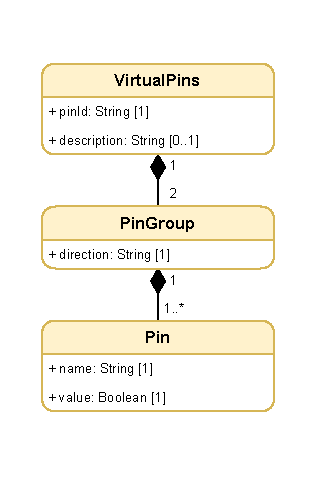
\includegraphics[width=0.4\textwidth]{5-Figures/VirtualPins.pdf}
    \caption{\gls{UML} Class Diagram of the \textit{VirtualPins} hierarchy (\textit{VirtualPins}, \textit{PinGroup}, and \textit{Pin}).}
    \label{fig:metamodel_signal_interface}
\end{figure}

The attributes across the \textit{VirtualPins} hierarchy (\Cref{fig:metamodel_signal_interface}) are:

\textbf{\textit{VirtualPins}:}
\begin{itemize}
    \item \textbf{\textit{pinId}} (\textit{String}, $[1]$): Unique identifier for this \gls{IO} terminal interface block.
    \item \textbf{\textit{description}} (\textit{String}, $[0..1]$): Optional documentation describing the hardware interface.
\end{itemize}

\textbf{\textit{PinGroup}:}
\begin{itemize}
    \item \textbf{\textit{direction}} (\textit{String}, $[1]$): Signal transmission direction: \textit{INPUT} for digital sensors sending state data from the plant, or \textit{OUTPUT} for actuation commands received by the asset.
\end{itemize}

\textbf{\textit{Pin}:}
\begin{itemize}
    \item \textbf{\textit{name}} (\textit{String}, $[1]$): The logical tag name or physical \gls{PLC}/\gls{IO} terminal address.
    \item \textbf{\textit{value}} (\textit{Boolean}, $[1]$): The instantaneous discrete boolean state of the electrical signal (\textit{true} for HIGH, \textit{false} for LOW).
\end{itemize}

Through this decoupling, \textit{VirtualPins} strictly reflects the live electrical state, while \textit{BehaviorMapping} interprets that state to orchestrate physical kinematics inside the simulation engine.


\subsection{ControlLogic Class}
\label{sec:model_control_logic}

The \textit{ControlLogic} class stores local control rules and interlocks inside the asset ($0..1$), as shown in the \gls{UML} Class Diagram in \Cref{fig:metamodel_control_logic}. With this class, machines can run local automated sequences without needing an external \gls{PLC}.

\begin{figure}[htbp]
    \centering
    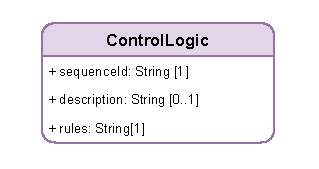
\includegraphics[width=0.4\textwidth]{5-Figures/ControlLogic.pdf}
    \caption{\gls{UML} Class Diagram of the \textit{ControlLogic} class.}
    \label{fig:metamodel_control_logic}
\end{figure}

The attributes of \textit{ControlLogic} are:
\begin{itemize}
    \item \textbf{\textit{sequenceId}} (\textit{String}, $[1]$): Unique identifier for the control sequence.
    \item \textbf{\textit{description}} (\textit{String}, $[0..1]$): Optional description of the sequence.
    \item \textbf{\textit{rules}} (\textit{String}, $[1]$): Text containing the conditional IF-THEN rules run by the simulation engine.
\end{itemize}

\subsection{NetworkEndpoint Class}
\label{sec:model_network_endpoint}

The \textit{NetworkEndpoint} class specifies the network protocol and address used to communicate with the physical equipment or data services ($0..1$). The structure of this interface is depicted in the \gls{UML} Class Diagram in \Cref{fig:metamodel_network_endpoint}.

\begin{figure}[htbp]
    \centering
    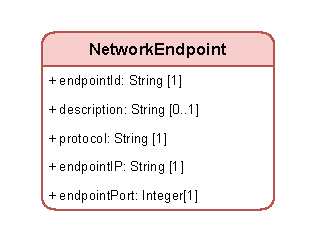
\includegraphics[width=0.4\textwidth]{5-Figures/NetworkEndpoint.pdf}
    \caption{\gls{UML} Class Diagram of the \textit{NetworkEndpoint} class.}
    \label{fig:metamodel_network_endpoint}
\end{figure}

The attributes of \textit{NetworkEndpoint} are:
\begin{itemize}
    \item \textbf{\textit{endpointId}} (\textit{String}, $[1]$): Unique identifier for this network interface.
    \item \textbf{\textit{description}} (\textit{String}, $[0..1]$): Optional description of the endpoint.
    \item \textbf{\textit{protocol}} (\textit{String}, $[1]$): Communication protocol (e.g., \gls{TCP} socket, \gls{HTTP} \gls{REST}, \gls{MQTT}).
    \item \textbf{\textit{endpointIP}} (\textit{String}, $[1]$): \gls{IP} address or hostname.
    \item \textbf{\textit{endpointPort}} (\textit{Integer}, $[1]$): Target port number.
\end{itemize}

\section{Chapter Summary and Architectural Transition}
\label{sec:architecture_summary}

This chapter established the conceptual foundation of the \gls{DT} framework. By formalizing four functional requirements (\textbf{FR1}--\textbf{FR4}) and four non-functional requirements (\textbf{NFR1}--\textbf{NFR4}) under the normative taxonomy of \textcite{Alemao2022}, the framework directly resolves the challenges of vendor lock-in, manual reconstruction, and synchronization drift. The architecture decouples asset authoring from runtime execution through three functional layers, backed by a vendor-neutral semantic metamodel that integrates 3D visual representations, kinematic definitions, virtual pin mappings, behavioral rule logic, and network endpoints into self-describing packages.

While this chapter focused on technology-agnostic specifications, the practical deployment of this architecture requires concrete software engineering choices, standards serializations, and physical hardware interfaces. \Cref{cha:implementation} details the technical implementation of this architecture, describing the realization of the modeling wizard in Python and PyQt6, the semantic repository using Eclipse BaSyx v2, the runtime simulation engine in Unity, and the real-time embedded firmware on industrial Arduino controllers.


